\documentclass{article}

\usepackage{graphicx}
\usepackage{amsmath}
\usepackage{caption}
\usepackage{subcaption}
\usepackage{listings}
\usepackage[hidelinks]{hyperref}
\usepackage{enumitem}
\usepackage{geometry}
\usepackage{biblatex}

\renewcommand{\contentsname}{Table of Contents}
\addbibresource{rdd.bib}

\begin{document}

\begin{titlepage}
\begin{center}
\vspace*{1cm}

\Huge
\textbf{Project 01: Home Safe}

\vspace{0.5cm}
\Large
\textit{Requirements Definition Document} \\
\textit{RDD Version 2}

\vspace{1cm}

\textbf{Team 01}

\vspace{0.5cm}

\text{Marina Seheon (Manager)} \\
\text{Andrei Phelps (Document Manager)} \\
\text{Luke McDougall (Lead Software Engineer)} \\
\text{Jack Vanlyssel} \\
\text{Spoorthi Menta} \\
\text{Vamsi Krishna Singara} \\

\vspace{1cm}

\begin{figure}[h]
    \centering
    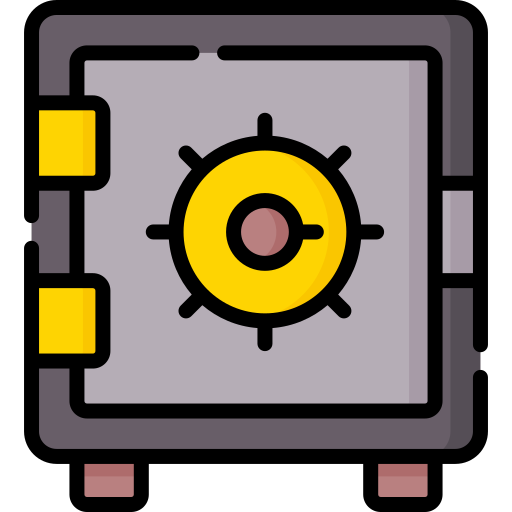
\includegraphics[width=0.25\textwidth]{docs/figs/safe.png}
    \caption*{Image courtesy of Flaticon.com \cite{flaticonSafeDeposit}.}
    \label{fig:safeIcon}
\end{figure}


\vspace{2.5cm}

\Large
\textbf{CS460: Software Engineering} \\

\end{center}
\end{titlepage}

\newpage

\tableofcontents

\newpage

\section{Introduction}
This document is a comprehensive guide to HomeSafe, a cutting-edge digital safe designed for unparalleled security and convenience. HomeSafe aims to revolutionize the safe industry with its innovative objectives, which include delivering a state-of-the-art digital safe that merges ease of use with robust security features. The system organization is meticulously planned, incorporating various technological components like retina scanners and integrated into its two-factor authentication mechanisms, making it highly secure yet accessible. One unique capability that sets HomeSafe apart is its multi-user accommodation feature, designed to be incredibly versatile and ideal for households with multiple users. \\ \\
The guide is organized into several crucial sections to give readers a thorough understanding of HomeSafe. These include the "Definition of Terms," which demystifies any technical language, and "Objectives," which explains HomeSafe's ambition to create a seamless blend of security and convenience. The "System Organization" section outlines the architectural components and integrated technologies like retina scanners that make the product unique and secure. "Capabilities" highlights the user-friendly interface and streamlined setup process, ensuring ease of use for everyone. Lastly, "Design Constraints" discusses power supply issues, size limitations, and data integrity concerns under specific scenarios. \\ \\
Despite the constraints, HomeSafe remains committed to its primary mission: providing exceptional security and convenience. Whether you're a stakeholder in the project or a consumer looking to better protect your valuable assets like money, jewelry, and crucial documents, this guide offers a comprehensive overview. It seeks to assure you that HomeSafe is a forward-thinking solution designed to meet the modern needs of safeguarding valuable possessions.

\section{Definition of Terms}
This section provides definitions for critical terms recurrently utilized throughout the document. This section can be a reference point for readers engaging with the content.

\begin{enumerate}
    \item[I.] \textbf{Auxiliary}: An additional or secondary power source that supports the main or primary power supply. An auxiliary power source is typically used to provide backup, redundancy, or temporary power when the main power source is unavailable, disrupted, or insufficient.
    \item[II.] \textbf{Bio-Metric Scanner}: A technology that identifies and authenticates users based on their unique biological characteristics, typically fingerprints, retina patterns, or other traits.
    \item[III.] \textbf{Central Processing Unit (CPU)}: Also known as a central processor or a main processor, it serves as the core component of any computer. This unit carries out the essential functions of executing program instructions, including tasks like calculations, logical operations, control functions, and managing input/output processes.
    \item[IV.] \textbf{Microcontroller}: A microcontroller is a small integrated circuit serving as the central processing unit (CPU) of a safe's electronic system. It contains a processor, memory, and input/output ports and can include programmable capabilities. Microcontrollers manage the safe's tasks, user input, security protocols, and control functions, including locks, interface interactions, and external device communication.
    \item[V.] \textbf{Personal Identification Number (PIN)}: A numerical code that serves as a security credential used to authenticate and verify the identity of an individual. PINs are commonly used in various systems, such as electronic devices, bank accounts, and access control systems, to ensure that only authorized users can gain access.
    \item[VI.] \textbf{Two-Factor Authentication (2FA)}: A security protocol that requires users to provide two distinct forms of verification to access a system. This commonly involves a combination of something known (such as a password), and something possessed (such as a generated code or biometric information), adding an extra layer of security and protection against unauthorized access \cite{identityautomationTwoFactorAuthentication}.
\end{enumerate}

\section{Objectives}
Our main goal is to develop a safe that can seamlessly accommodate multiple individual users, each with independent access. The design prioritizes ease of setup and maintenance, showcased through a user-friendly interface that facilitates straightforward management and configuration. Enhanced security is another core objective, achieved through implementing Two-Factor Authentication, which includes a biometric retina scan. Even in the face of power outages, our focus on security ensures that user data remains intact, reinforcing our commitment to offering convenient access and robust protection.

\subsection{Multi-User Capability}
The safe comes with a multi-user feature, allowing for the storage of unique access codes for each user. This enables independent access for multiple individuals, whether in a household or an organization, without compromising the system's overall security. Each user's code is securely encrypted, maintaining a high level of protection for everyone. This feature adds an extra layer of convenience, making the safe versatile and well-suited for various settings.

\subsection{Enhanced Security with Two-Factor Authentication}
Two-factor authentication (2FA) is integrated into the safe for enhanced security, using a predetermined 2FA code shipped with the safe. Upon initial setup, the safe will require the user's unique code and the provided 2FA code for access. The user will then be prompted to provide a biometric retina scan to complete the setup for their access. This built-in dual-layer authentication significantly boosts the security of the safe, making it more challenging for unauthorized individuals to gain access.

\subsection{Easy Setup and Care}

When you receive HomeSafe, the setup process is made smoother with pre-installed batteries, eliminating the requirement for extra assembly. The unit is meticulously designed for user-friendly operation: just power on the safe and follow the straightforward prompts to finalize the setup. This method guarantees a seamless experience from the beginning, reducing user involvement and erasing the usual intricacies linked to initial installation.

\subsection{Uninterrupted Security and Access}
In a power outage, the safe has an auxiliary CR2032 battery to keep the microcontroller and all user data secure and intact. This safety measure underscores our commitment to maintaining data integrity and security, even during unexpected power interruptions.

\section{System Organization}
This section provides a comprehensive overview of the HomeSafe system's architecture, breaking down its user interface, interior design, and the seamless interaction between its components.

\subsection{User Interface}
The user interface combines multiple elements, including a numeric keypad, specialized keys, an LED display, an iris scanner, and a speaker for auditory feedback. These elements are meticulously designed to ensure an easy-to-use, secure authentication process.

\vspace{0.3cm}

\

\begin{center}
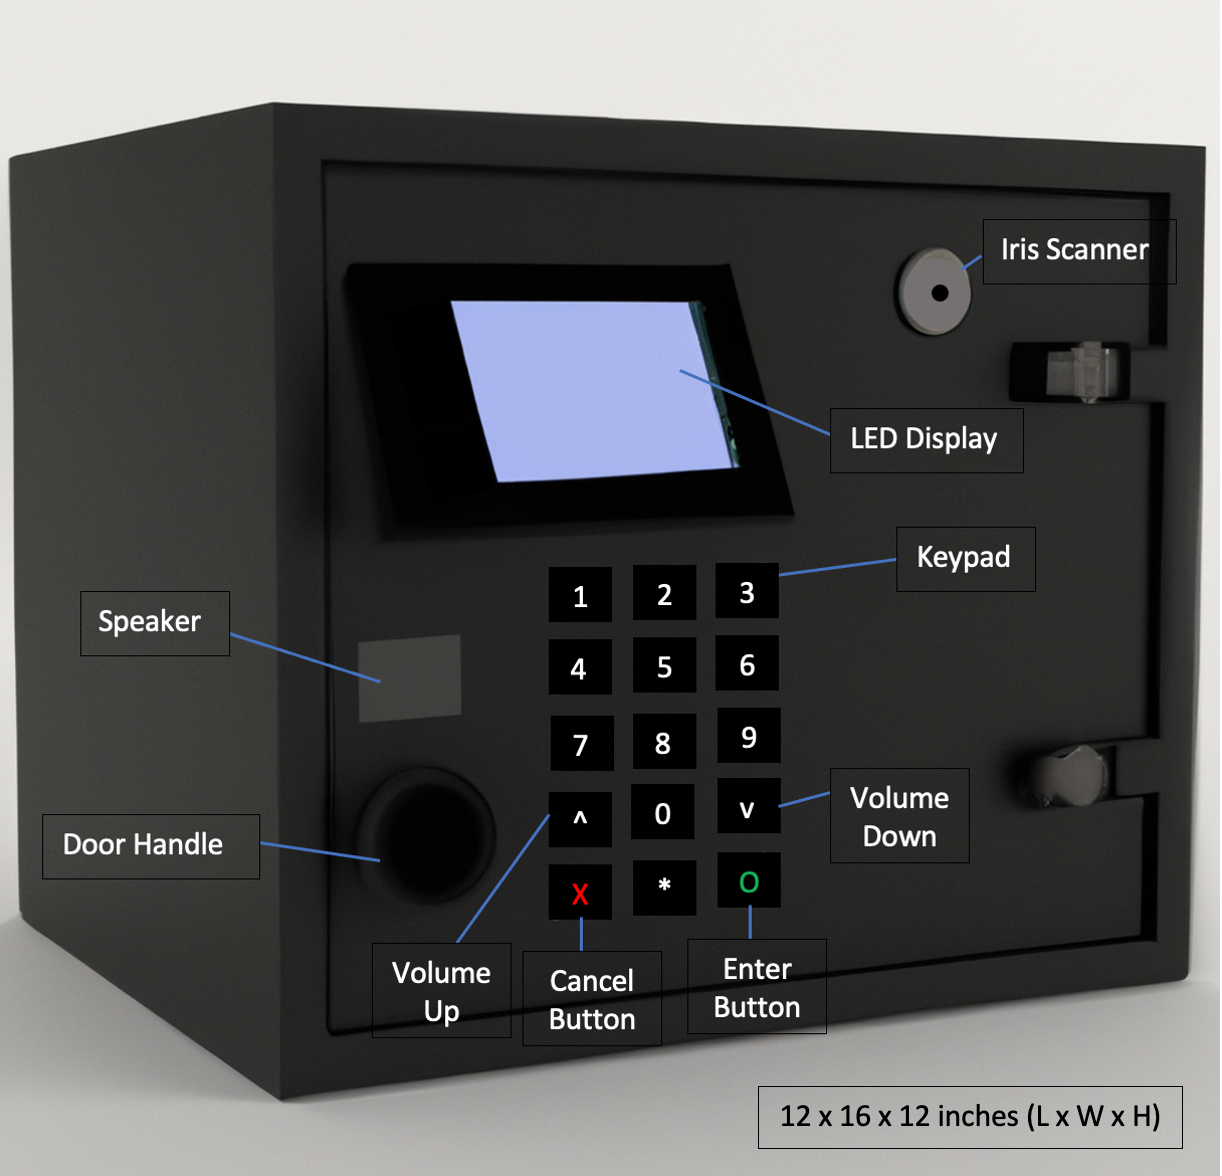
\includegraphics[scale=0.55]{docs/figs/closed_safe.png}
\end{center}

\begin{enumerate}
    \item \textbf{Keypad}: The secondary source of authentication. Once the bio-metric scan is complete, users must input their six-digit PIN using the number keys labeled 0-9. If the user enters an incorrect PIN or lets more than three seconds elapse after input, the system will reset the user's attempt. After three failed attempts, the user will be restricted access and need an administrator's PIN to regain access.
    \item \textbf{Red X Key}: If a user makes an incorrect entry during PIN entry, they can press this button to reset their attempt. This will not be counted as a failed attempt.
    \item \textbf{Green Circle Key}: The user must press this button after entering all six digits of their PIN. Upon pressing this button and entering the correct PIN, the latches will be released, allowing the user access.
    \item \textbf{LED Display}: The display screen acts as an interactive interface between the user and the safe. Each time a key is pressed for password entry, an asterisk (*) appears on the screen to indicate the number of digits entered. This feature is designed to enhance user experience by providing real-time feedback.
    \item \textbf{Iris Scanner}: The primary source of authentication. Once the user provides a retinal scan, the microcontroller will enable communication with the keypad. This will prompt the user to input their six-digit code using the keypad on the LED Display.
    \item \textbf{Speaker}: Provides auditory feedback to the user when interacting with the user interface.
    \item \textbf{Volume Buttons}: The user can increase or decrease volume levels.
    \item \textbf{Power Button}: Powers the system on or off when pressed. \textbf{NOTE}: The system cannot be powered off if the locking mechanism is unlocked (safe door is open position).
    \item \textbf{Door Handle}: Used to open the safe once the latches have been released after successful authentication.
\end{enumerate}

\subsection{Interior Design}
In this section, we explore the internal architecture of HomeSafe, focusing on its quality materials and advanced technologies. The safe's interior is cushioned with a foam base to protect delicate items, while twin steel latches ensure secure locking. Lock sensors and a microcontroller work together to manage the safe's status, making it both smart and secure. The system runs on two AA batteries in a dedicated compartment, with a backup CR2032 cell battery for uninterrupted operation. These components are integrated seamlessly to offer a reliable, user-friendly safe for safeguarding your valuables.

\vspace{0.3cm}

\begin{center}
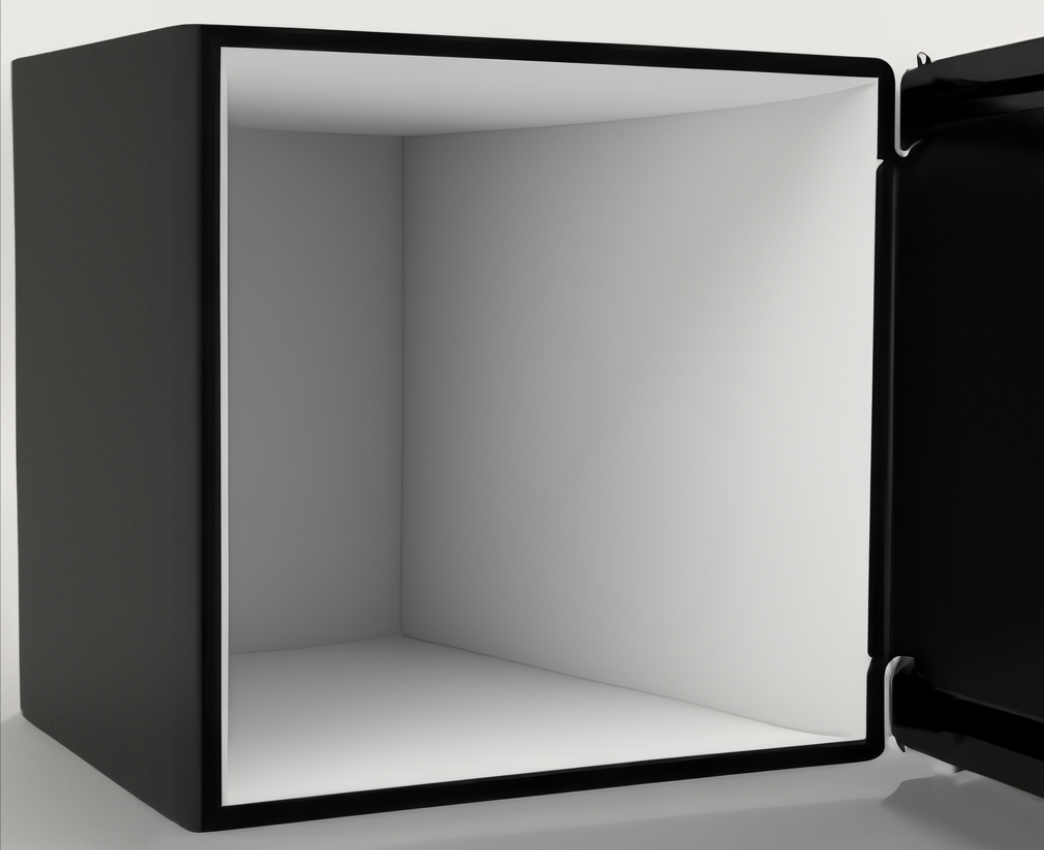
\includegraphics[scale=0.55]{docs/figs/open_safe.png}
\end{center}

\begin{enumerate}
    \item \textbf{Foam Interior Base}: A soft foam base that covers the steel floor of the safe. This allows for the safe storage of otherwise delicate items.
    \item \textbf{Steel Latches}: While the safe is locked, the twin steel latches press down on the lock sensors.
    \item \textbf{Lock Sensors}: Communicates with the microcontroller whether the safe is in the locked or unlocked state.
    \item \textbf{Micro-Controller}: Powered by the batteries, this is where the system's brains are housed. Inputs are received and interpreted before sending any output to the user. Requires power to store user data such as PINs, bio-metric, and user data \cite{gridling2007introduction}.
    \item \textbf{Battery Compartment}: Compartment where the primary power source, two AA batteries, is stored.
    \item \textbf{Auxiliary Power}: The secondary power source is stored inside the microcontroller, a single CR2032 cell battery.
\end{enumerate}

\section{Capabilities}
HomeSafe is engineered to balance user convenience with cutting-edge security measures perfectly. It supports the creation of up to six individual profiles, each equipped with its unique PIN and Two-Factor Authentication biometric data. This multi-layered approach minimizes the chances of unauthorized entry. To further enhance the user experience, HomeSafe arrives with batteries pre-installed, facilitating a smooth setup process. Its intuitive user interface simplifies initial configuration and ongoing use, positioning HomeSafe as a dependable, secure, and hassle-free option for protecting your valuables.

\subsection{Multi-User Capability}
The Multi-User Capability feature amplifies ease of use and quick access for multiple users, fostering smooth and efficient collaboration.

\begin{itemize}
    \item \textbf{User Profiles}: Generate up to six individual user profiles in the system, each featuring a unique PIN and biometric Two-Factor Authentication information.
\end{itemize}

\subsection{Enhanced Security with Two-Factor Authentication}
Achieve heightened security and peace of mind with Two-Factor Authentication, which includes the crucial component of a retina scanner as part of the verification process.

\begin{itemize}
    \item \textbf{Advanced Security}: Implementation of two-factor authentication significantly fortifies security measures, ensuring unauthorized access is thwarted.
    \item \textbf{Comprehensive Access Control}: Incorporating multiple verification factors allows for more comprehensive control over who can access the system.
    \item \textbf{Reduced Vulnerability}: Enhanced security through 2FA reduces vulnerability to hacking, phishing, and other malicious activities.
\end{itemize}

\subsection{Easy Setup and Care}
This robust set of features ensures the system's reliability, ease of use, and continual security, aligning perfectly with the goal of efficient, user-friendly operation.

\begin{itemize}
    \item \textbf{Hassle-Free Setup}: The unit is equipped with pre-installed batteries, streamlining the installation process by removing the step of battery setup. It functions entirely on battery power, so there's no requirement for an AC connection. Just turn on HomeSafe and follow the on-screen instructions for a quick setup.
    \item \textbf{Intuitive Interface}: Design a user-friendly interface that effortlessly guides users through the setup process.
\end{itemize}

\subsection{Uninterrupted Security and Access}
Strengthening seamless security and access, these integrated features form the cornerstone of sustained operational reliability, bolstering the system's trustworthiness across various circumstances.

\begin{itemize}
    \item \textbf{Backup Power Integration}: Integrated auxiliary power source that seamlessly takes over when the main battery depletes.
    \item \textbf{Advanced Low-Battery Alerts}: Provide early notifications to users when the battery level drops, enabling them to take proactive measures.
    \item \textbf{Emergency Power Reserve}: Designate a portion of the battery capacity as an emergency reserve, ensuring critical operations can continue even if the battery is almost depleted.
\end{itemize}

\section{Design Constraints}
While HomeSafe prioritizes user-friendliness and robust security, there are some inherent design limitations to be aware of:

\begin{itemize}
    \item The system allows for PIN codes that are six digits in length. This may limit the level of complexity for user codes, and users are encouraged to avoid easily guessable combinations like 1, 2, 3, 4, 5, and 6.
    \item HomeSafe relies on two AA batteries for its primary power source. If these batteries deplete, the system automatically shifts to an auxiliary CR2032 battery housed within the microcontroller. This ensures that your settings and user data remain intact even when the primary batteries are exhausted.
    \item HomeSafe operates exclusively on batteries, so it cannot be connected to an external power source like an AC adapter. This needs to be considered for long-term maintenance.
    \item The auxiliary power supply can power the system for approximately ten years \cite{microbatteryEverythingNeed}. If the auxiliary power supply is depleted before the primary power supply is restored, all user data will be lost, and the unit's contents will not be accessible.
    \item With external dimensions of 12 x 16 x 12 inches (L x W x H), the HomeSafe offers a finite amount of storage space. Users should consider these dimensions when planning what to store inside the safe.
    \item Two-Factor Authentication (2FA) is activated through a predetermined code shipped with the safe. While this enhances security, users should keep this code secure and confidential.
    \item HomeSafe is not designed to be fireproof or waterproof. Users should consider the safe's environmental limitations when choosing a location.
    \item All images of the safe were created using the DALL-E 2 generative AI technology by OpenAI \cite{openaiDALLE}. We added labels and arrows to each safe component using Microsoft Word.
\end{itemize}

\newpage

\printbibliography

{\parindent0pt}

\end{document}
